\chapter{Testing}

%Detailed descriptions of every test case are definitely not what is required here. What is important is to show that you adopted a sensible strategy that was, in principle, capable of testing the system adequately even if you did not have the time to test the system fully.

%Have you tested your system on 'real users'? For example, if your system is supposed to solve a problem for a business, then it would be appropriate to present your approach to involve the users in the testing process and to record the results that you obtained. Depending on the level of detail, it is likely that you would put any detailed results in an appendix.

\section{Overall Approach to Testing}
As this is a research-based project, it is difficult to perform any for of unit, functional or 
requirements testing. Most testing is based on validating the results of analysis and 
classification techniques.


\section{Validation}
Cross-validation is a statistical concept used to assess how the results of statistical analysis
generalise to an independent data set. Cross-validation is typically applied to machine learning
classifiers to test if a technique is overfitting the data; that is how specific the technique is
to the original data set and how it can cope with new examples. For example, a rote learner cannot
classify any unseen examples as the classification is performed based solely on the training set.

As the overall goal is to be able to classify any Williams painting it is important that the 
program is able to handle new examples, not just those for which the year is known.

There are many forms for calculating cross-validation, usually involving taking sub-samples of the
original data set and removing them from the training set to create a validation set.

$k$-fold cross-validation is a common method for performing this. It involves splitting the data
set into $k$ sections or \emph{fold}. Each fold is removed from the data set, the classifier is
trained on the remaining data, then the fold is classified using the trained data. 

The other common form of cross-validation is to take random sub-samples from the data set and are
removed from the training set and then classified using it. This process is performed repeatedly
until a good number of samples has been taken. This has advantages and disadvantages over $k$-fold
cross-validation, it has the problem that not all data points are considered during validation,
but doesn't depend on the size of the data set.


\subsection{Leave-One-Out Cross-Validation}
Leave-one-out cross-validation is a form of $k$-fold cross-validation in which the number of folds
is equal to the size of the data set. This leads to the behaviour of leaving a single data point
each time and classifying it against the rest of the data set. Because data sets in machine 
learning are typically very large this usually isn't an option due to time complexity.

However, because of the use of $k$-Nearest Neighbour-based classifiers (which need no re-training 
when data points are added or removed) and a small number of known data points, it is the best 
method of cross-validation for this project.

Leave-one-out cross-validation provides us with a classified year for each data point and, because
we only use data points with known years, we can then work out the correlation between actual and
classified years to get a value of performance.

To produce this value Pearson's product-moment correlation was used (equation~\ref{eq:pearsons})
the best techniques would produce a correlation value closer to $1$ than other techniques. Another
part of Pearson's is that it is easy to generate statistical significance (the p-value). This
describes the extent to which the observations could appear by chance in a given single null
hypothesis.

The results of the correlation between actual and classified year is defined to be $r$ 
(formally: $r=\rho_{classified, actual}$). The p-value is defined to be $P(r)$. The ultimate goal 
being to maximise $r$ whilst minimising $P(r)$.

Of course, an exact correlation of $r=1$ would be unrealistic to achieve, especially for such a 
humanities-based project. A good technique might reach correlations of $r \ge 0.5$ and a great
technique might reach correlations of $r \ge 0.75$.

\section{Results}

One parameter for our classifier is the choice of $k$ for $k$-Nearest Neighbour. Simply setting 
$k=1$ has the effect of assigning the year of the nearest painting in feature space to the current
test painting, whilst setting $k=102$ has the effect of giving the painting the mean year of the 
entire data set. Obvious, a point between the two is likely to be the best. 

\begin{figure}[h]
\centering
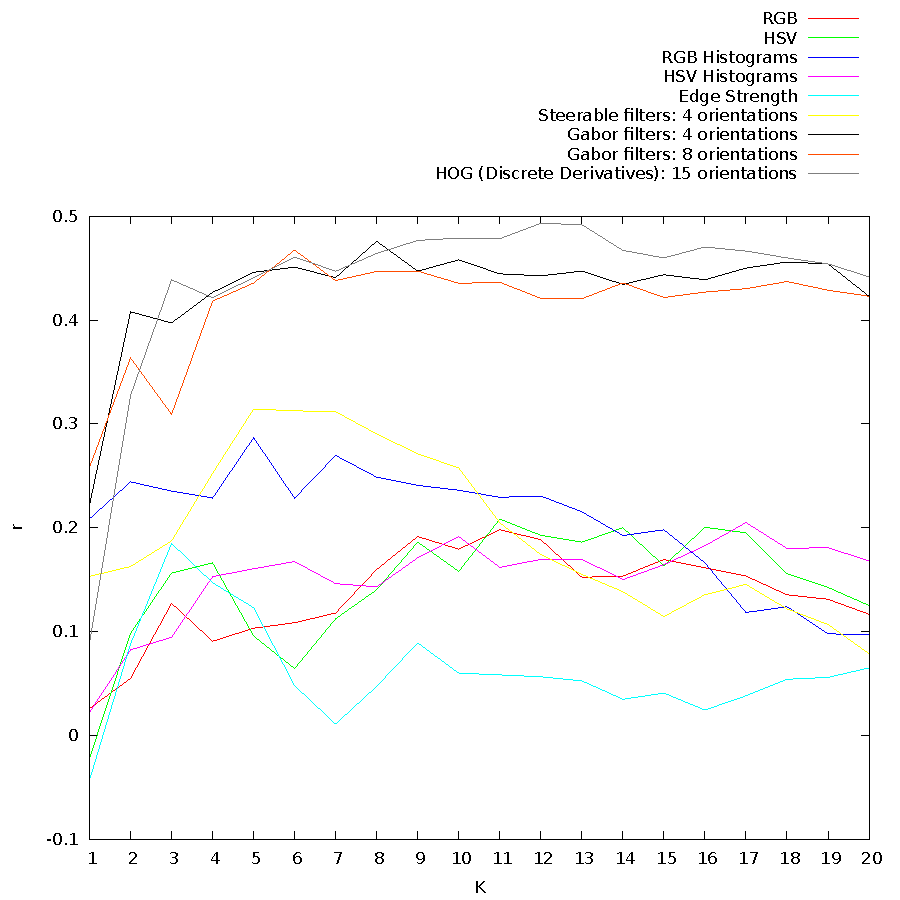
\includegraphics[width=0.9\textwidth]{../../isispa-paper/results/mean}
\caption{Correlation Coefficients $r$ against $k$ values for $k$-Nearest Neighbour}\label{fig:r-graph}
\end{figure}

From figure~\ref{fig:r-graph} it is apparent that for many of the features spaces we have that the 
optimum value of $k$ is around 7 or 8. Table~\ref{tab:r-results} shows the actual results for each 
feature space for a $k$ of 7, where $r$ is the correlation coefficient given by Pearson's, 
$P(r)$ is the p-value significance of $r$.

$C(n)$ is the percentage of paintings correctly classified within $n$ years of the actual year 
(where $E(X)-n \le X \le E(X)+n$).

\begin{table}[h]
\centering
\begin{tabular}{|l|c|c|c|}\hline
Technique     					& $r$    & $P(r)$ & $C(15)$ \\ \hline
Edge Strength 					& 0.0107 & 0.910  & 60\%    \\
HSV 						& 0.112	 & 0.237  & 64\%    \\
RGB 						& 0.118  & 0.214  & 63\%    \\
HSV Histograms					& 0.146	 & 0.123  & 64\%    \\
RGB Histograms					& 0.270	 & 0.004  & 62\%    \\
HOG (Discrete Derivatives): 4 orientations 	& 0.307	 & 0.001  & 65\%    \\
Steerable filters: 4 orientations 		& 0.312	 & 0.001  & 68\%    \\
HOG (Discrete Derivatives): 8 orientations 	& 0.346	 & \textless0.001 & 65\% \\
HOG (Discrete Derivatives): 16 orientations 	& 0.367	 & \textless0.001 & 64\% \\
Gabor filters: 16 orientations			& 0.370  & \textless0.001 & 67\% \\
Gabor filters: 8 orientations			& 0.438	 & \textless0.001 & 70\% \\
Gabor filters: 4 orientations			& 0.441	 & \textless0.001 & 71\% \\
\hline
\end{tabular}
\caption{Correlation Coefficients, ordered by strength for $k=7$}\label{tab:r-results}
\end{table}


\newpage
\subsection{Ensemble Results}
Using ensemble methods can both improve and weaken the correlation coefficients depending on the
techniques used. The inclusion of colour histogram analysis and HSV colour-space statistical
analysis typically weakens the results, whilst combining \gls{hog} and Gabor filters typically 
improves the correlation coefficients beyond each technique individually. 
Table~\ref{tab:ensemble-results} shows some examples of this.

This does show that ensemble methods can help to improve the strength of analysis techniques, as
expected.

\begin{table}[h]
\centering
\begin{tabular}{|l|c|c|}\hline
Method	& $r$	& $P(r)$ \\ \hline
RGB 						& 0.118  & 0.214 \\
Ensemble RGB Histogram and HOG (16)		& 0.256 & 0.006 \\
RGB Histograms					& 0.269 & 0.004 \\
HOG (Discrete Derivatives): 16 orientations	& 0.367 & \textless0.001 \\
Ensemble RGB and HOG (16)			& 0.372 & \textless0.001 \\
Gabor filters: 4 orientations			& 0.441 & \textless0.001 \\
Ensemble RGB and Gabor (4)			& 0.443	& \textless0.001 \\
Ensemble RGB, Gabor (4) and HOG (16)		& 0.464	& \textless0.001 \\
\hline
\end{tabular}
\caption[Correlation Coefficients comparing individual and ensemble methods]{Correlation Coefficients comparing individual and ensemble methods. Note how the 
combination of RGB Histograms and \gls{hog} has decreased performance, whilst the combination of
\gls{hog} and Gabor filters has improved performance.}\label{tab:ensemble-results}
\end{table}

\newpage
\section{Exemplar Results}
The intuition -- that using artistically chosen exemplars could help to exploit knowledge about 
the way the paintings change over time -- turned out to be incorrect; results for Gabor filters 
with 4 orientations (the best performing method in our previous experiment) are shown in 
Table~\ref{artistic_exemplars}.  Results for the other feature spaces show a similar pattern, the 
same distance measure ($\chi^2$) has been used throughout. 

\begin{table}[h]
\centering
\begin{tabular}{|p{3.5cm}|c|c|c|}
\hline
Technique     & $r$ & $P(r)$ & $C(15)$ \\ \hline
%K=7
Artistic Exemplars	& 0.328	& \textless0.001 & 57\%\\
Statistical Exemplars	& 0.383	& \textless0.001 & 61\%\\
Centroid		& 0.403	& \textless0.001 & 64\%\\
\hline
\end{tabular}
\vspace{0.5em}
\caption{Correlation coefficients, ordered by strength, for Exemplars
\label{artistic_exemplars}}
\end{table}

These exemplars give an interesting insight into the feature space. The paintings shown in 
Figures~\ref{early_example} and~\ref{late_example} are both artistic exemplars, however the 
earlier painting ``\emph{Snowdon, the Traeth and the Frightened Horse}'', from 1948, is far from 
the feature space centroid for that year, whereas the later painting is very close to the feature 
space centroid for 1985. A visualisation of artistic exemplars and their corresponding statistical
representations is given in Figure~\ref{art_ex_stat_ex}. From this you can see that artistic 
information does not necessarily correspond well to the feature space(s) we use. Note that whilst 
Figure~\ref{art_ex_stat_ex} uses the feature space defined by Gabor filters with 4 orientations, 
our best performing: the pattern is similar for all other feature spaces.

\begin{figure}[h]
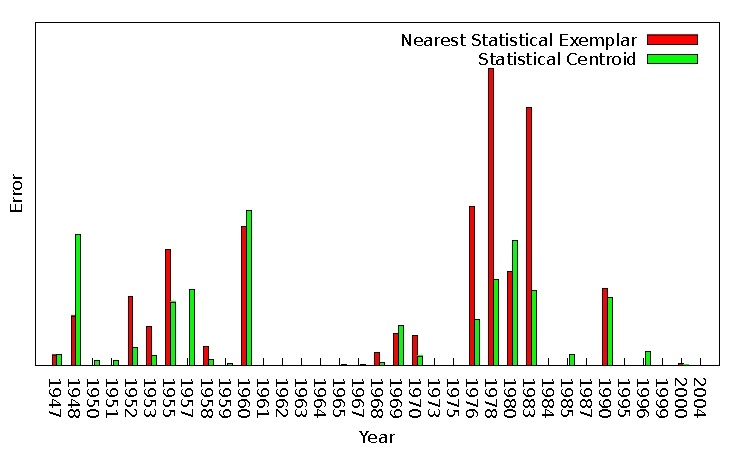
\includegraphics[width=\linewidth]{img/exemplar.pdf}
\caption[Distance in feature space from artistic to statistic exemplars]{Distance in feature space from artistic to statistic exemplars (red); distance from 
artistic exemplar to centroid (green). Lower values indicate that the artistic exemplar is near to
the mean painting for a particular year, higher values that an artistic exemplar painting is an 
outlier for this particular feature space\label{art_ex_stat_ex}}
\end{figure}


%\subsection{Validation using Weka}

